\documentclass{standalone}
\usepackage{tikz}
\usepackage{pgfplots}
\pgfplotsset{width=16cm,height=18cm,compat=1.3}
\pgfplotsset{every tick label/.append style={font=\Huge}}
\usepackage{filecontents}
\usepgfplotslibrary{fillbetween}

\usetikzlibrary{patterns}

\definecolor{citrine}{rgb}{0.89, 0.82, 0.04}
\definecolor{arylideyellow}{rgb}{0.91, 0.84, 0.42}
\definecolor{bronze}{rgb}{0.8, 0.5, 0.2}

\begin{document}
	\centering
		\vspace{1.5em}
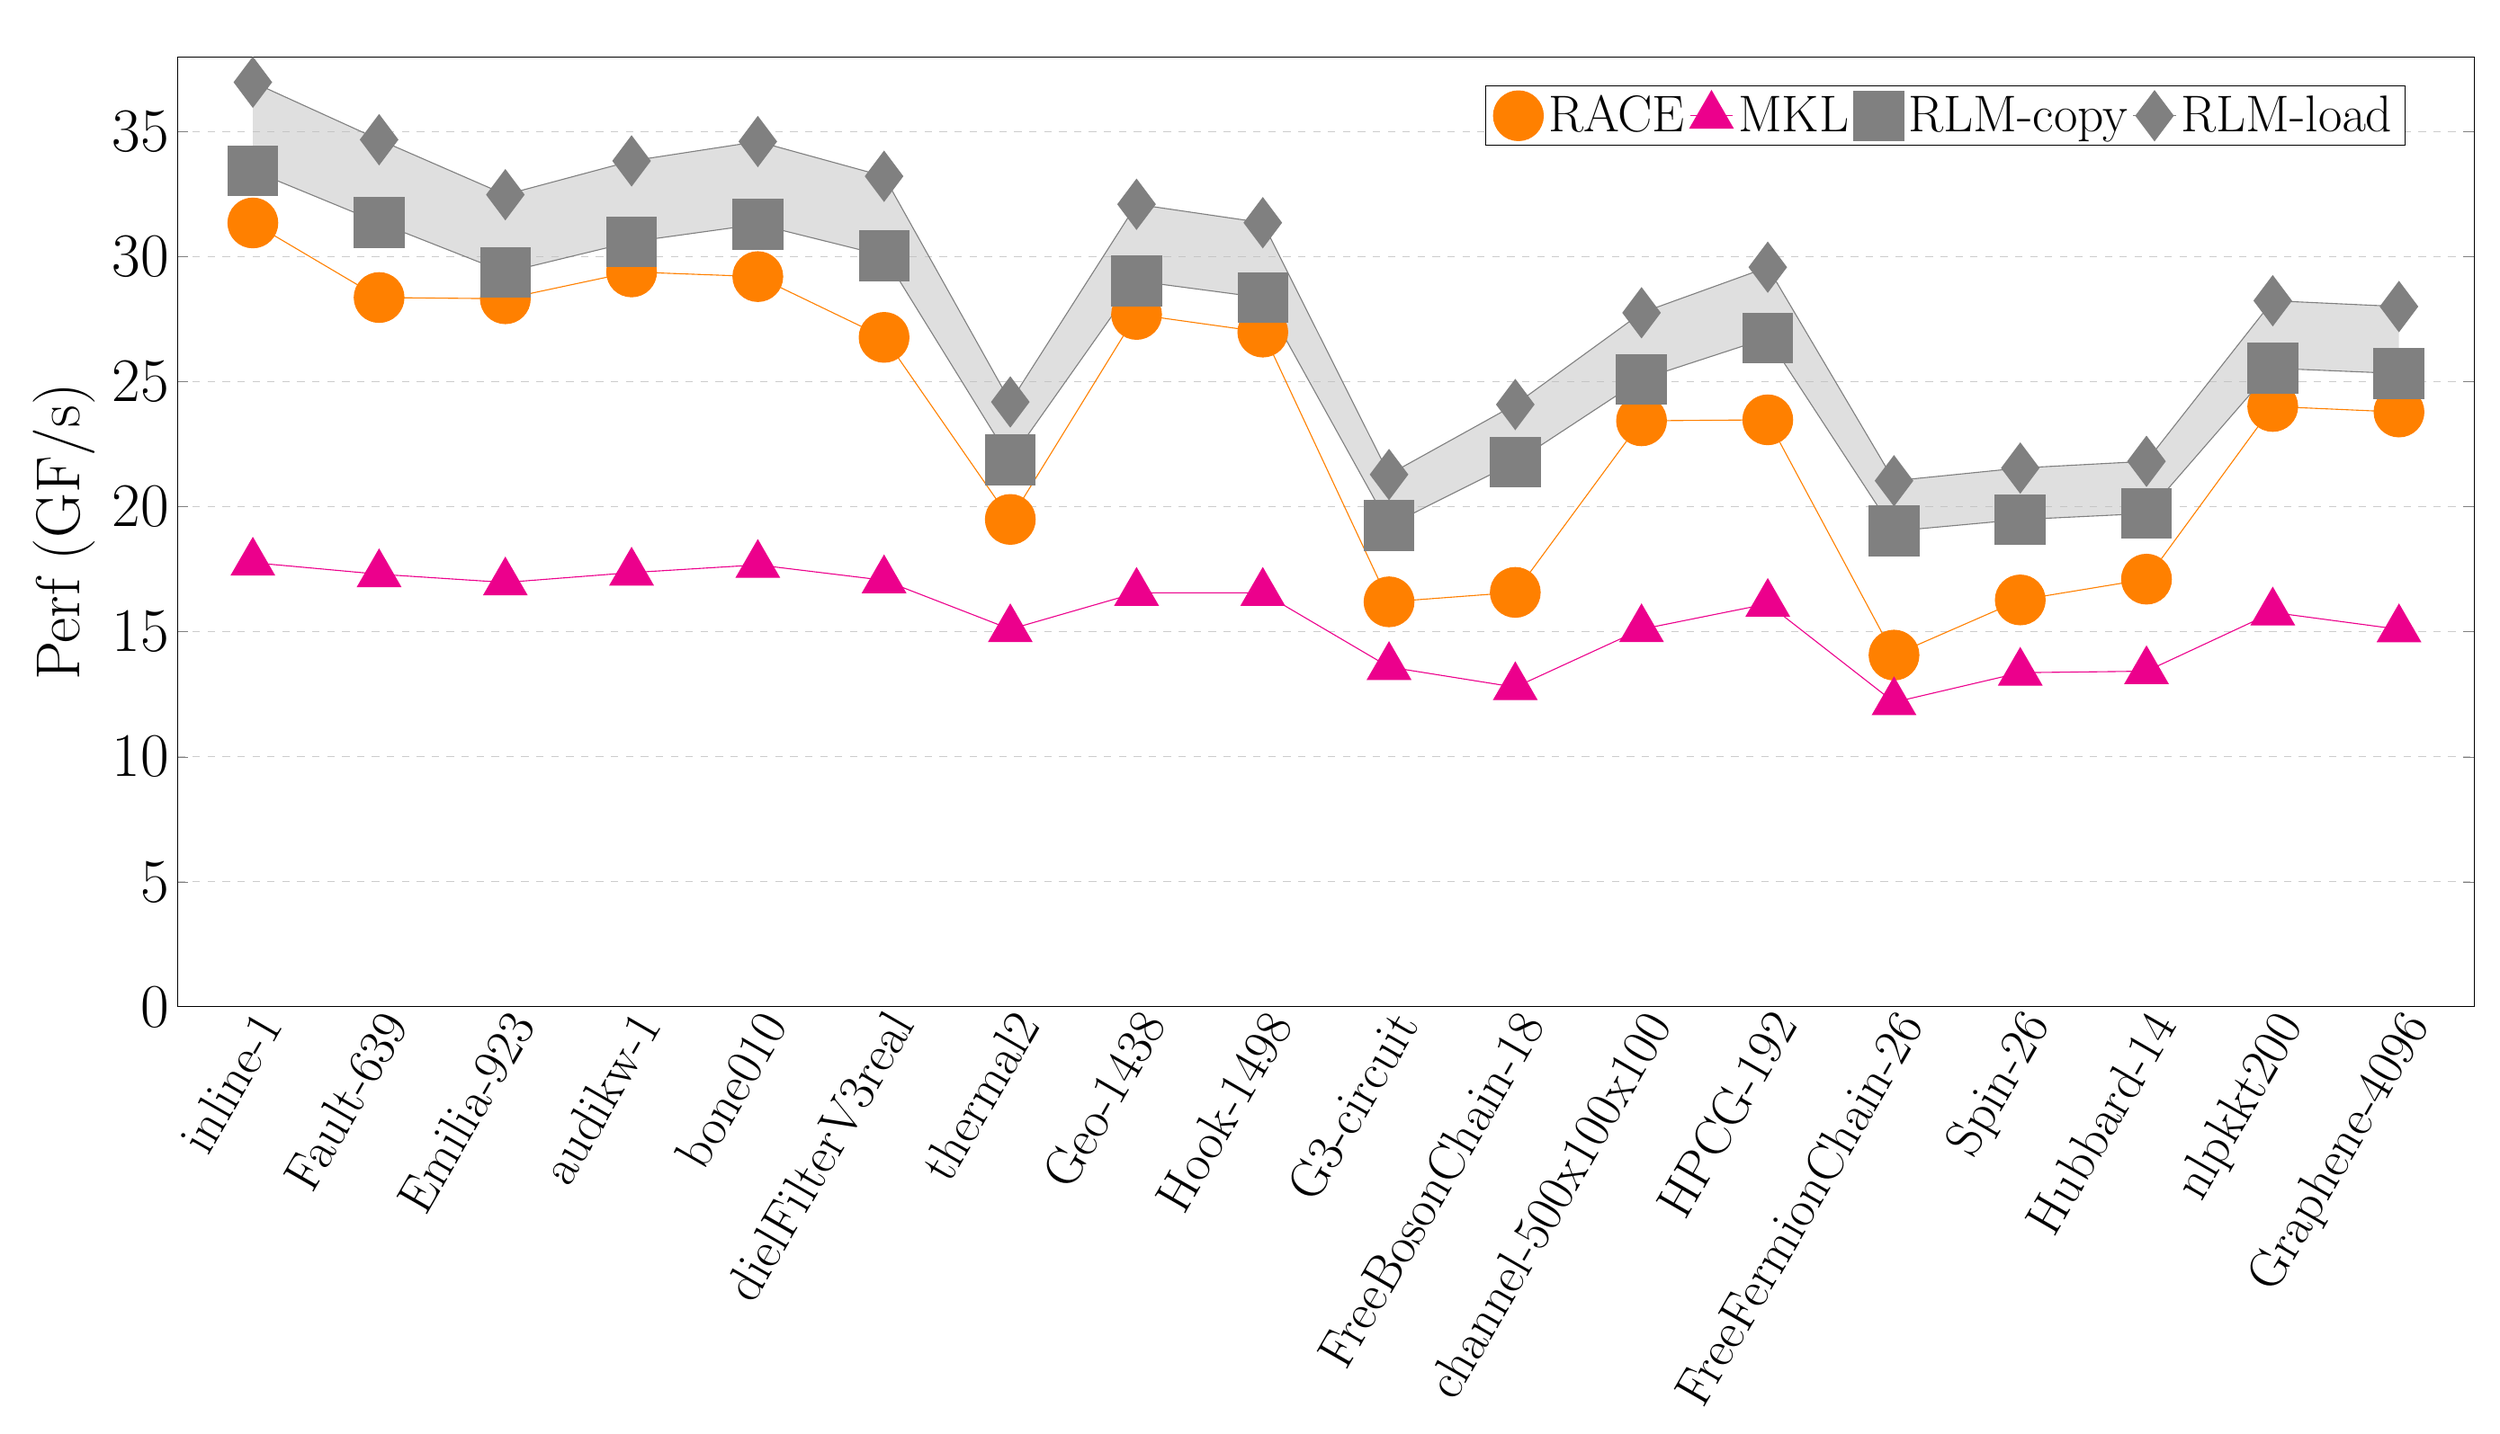
\begin{tikzpicture}
		%	\node at (13.25,15) {\LARGE{}};
			\begin{axis}[
		%	xmin=0.25, xmax=7.25,
			ymin=0, %ymax=3.25,
			ymax=38,
			xtick={1, 2, 3, 4, 5, 6, 7, 8, 9, 10, 11, 12, 13, 14, 15, 16, 17, 18},
		%	ytick={0,0.5,1,1.5,2,2.5,3},
			xticklabels={ inline-1, Fault-639, Emilia-923, audikw-1, bone010, dielFilterV3real, thermal2, Geo-1438, Hook-1498, G3-circuit, FreeBosonChain-18, channel-500x100x100, HPCG-192, FreeFermionChain-26, Spin-26, Hubbard-14, nlpkkt200, Graphene-4096},
			width  = 34cm,
			height = 15cm,
			major x tick style = transparent,
			%	minor ytick={1, 5, 10, 15, 20, 25, 30 ,35,40},
			grid = minor,	
			%add_bar_commands
			ymajorgrids = true,
			grid style={dashed, gray!40},
			ylabel = {\Huge{Perf (GF/s)}},
		%	symbolic x coords={Graphene-2048-2048, Graphene-4096-4096, Spin-24-24-24},
			x tick label style={rotate=60, anchor=north east, inner sep=0mm, font={\huge}},
		%	tick label style={font={\Huge}},
			scaled y ticks = false,
			enlarge x limits=0.035,
			legend cell align=left,
			legend style={font=\huge},
			legend columns=-1,
			legend style={
				%at={(1,1.05)},
				%anchor=south east,
				%column sep=1ex,
				legend pos=north east
			},
			%spl_legend_code
			title= {\Huge\scalebox{1.5}{{}}}
			]
\addplot[name path=RACE-SymmSpMV, mark=*, mark size=10pt, mark options={orange}, draw=orange ] plot coordinates{(1,31.356939) (2,28.372987) (3,28.323231) (4,29.396679) (5,29.210280) (6,26.778583) (7,19.496395) (8,27.696097) (9,26.990050) (10,16.199662) (11,16.577436) (12,23.441453) (13,23.480804) (14,14.069287) (15,16.275497) (16,17.107030) (17,24.014713) (18,23.793009)};
\addplot[name path=MKL-SymmSpMVIE, mark=triangle*, mark size=10pt, mark options={magenta}, draw=magenta] plot coordinates{(1,17.767401) (2,17.304731) (3,16.975884) (4,17.369550) (5,17.678201) (6,17.062434) (7,15.104626) (8,16.560236) (9,16.560155) (10,13.593018) (11,12.785401) (12,15.105072) (13,16.121380) (14,12.183172) (15,13.365014) (16,13.425972) (17,15.776211) (18,15.101306)};
\addplot[name path=RLM-copy, mark=square*, mark size=10pt, mark options={gray}, draw=gray ] plot coordinates{(1,33.448600498754566) (2,31.369144841935526) (3,29.379078942831114) (4,30.601322242191323) (5,31.302577971608205) (6,30.046007594627486) (7,21.88158503049584) (8,29.03360063990211) (9,28.36529966442702) (10,19.257114640970986) (11,21.788631100011006) (12,25.107708815137492) (13,26.75615029292358) (14,19.030557606095222) (15,19.49194495374786) (16,19.734157095876782) (17,25.54372630375391) (18,25.33332832179717)};
\addplot[name path=RLM-load, mark=diamond*, mark size=10pt, mark options={gray}, draw=gray ] plot coordinates{(1,36.98643324381514) (2,34.68703516175563) (3,32.486481523322865) (4,33.83800055626925) (5,34.61342756475907) (6,33.2239507055977) (7,24.195983447182904) (8,32.10446224604561) (9,31.365475590472187) (10,21.293924843381376) (11,24.09319785097371) (12,27.763331862892418) (13,29.586127727752036) (14,21.04340504520145) (15,21.553592977701964) (16,21.821423711786828) (17,28.245466585881726) (18,28.012814971218024)};
\addplot[fill=lightgray,opacity=0.5]
fill between[of= RLM-copy and RLM-load];
	%addplot cmd

	\legend{RACE, MKL, RLM-copy, RLM-load}

	\end{axis}			
\end{tikzpicture}

\end{document}

